\documentclass{book}
\usepackage[english]{babel}
\usepackage[utf8]{inputenc}
\usepackage{graphicx}
\usepackage{subfigure}
\usepackage{float}
\usepackage{smartdiagram}
\usepackage{biblatex} 
\usepackage[linesnumbered, ruled,vlined, commentsnumbered]{algorithm2e}
\usepackage{tabularx}
\usepackage[english]{babel}
\usepackage{hyperref}

\hypersetup{
    colorlinks=true,
    linkcolor=black,
    filecolor=magenta,      
    urlcolor=cyan,
}
\urlstyle{same}
\pagestyle{empty}
\addbibresource{sample.bib} %Import the bibliography file
\graphicspath{{img/}}
\author{Fabiana Ritorti - Francisco Payes - Luigi Arena - Marsha Gomez Gomez}
\date{\today}

% --------------------------------------------------------------------

\begin{document}
    \begin{titlepage}
        \centering
        
\includegraphics[width=6cm]{unipi}
        \vfill
        \vspace{1.5cm}
        {\huge\textsc{Project report of K-means Algorithm Hadoop and Spark}\par}
        {\Large
            Department of Information Engineering\\
            Cloud Computing Project\\
            2020\\
            \vspace{5cm}
            F. Ritorti \\  F. Payes \\  M. Gomez\\ L. Arena 
            \vspace{2cm}
            \today
        }    
        \vfill
        \vfill
    \end{titlepage}
    
    \tableofcontents

% --------------------------------------------------------------------
\hypersetup{
    colorlinks=true,
    linkcolor=blue,
    filecolor=magenta,      
    urlcolor=cyan,
}
\urlstyle{same}

\chapter{Introduction}
    \section{The basic Idea}
    \paragraph{}   
	K Means is one of the most popular \textit{clustering algorithms}. K means stores k centroids that it uses to define clusters. A point is considered to be in particular cluster if it is closer to that cluster's centroid than any other centroid. 

 	K Means finds the best centroids by alternating between (1) assigning data points to clusters based on the current centroids (2) choosing centroids (points which are the center of a cluster) based on the current assignment of data points to clusters. 

\chapter{Design}\label{chap:design}
    \section{Dataset}
    \paragraph{}

    We use a \href{https://www.kaggle.com/julianjose/minute-weather}{Kaggle Weather Dataset} that contains weather data captured for a one-minute interval. This data comes from a weather station located in San Diego, California. The weather station is equipped with sensors that capture weather-related measurements such as air temperature, air pressure, and relative humidity. Data was collected for a period of three years, from September 2011 to September 2014, to ensure that sufficient data for different seasons and weather conditions is captured. 

    This weather dataset contains more than one million and a half of registers with thirteen fields that consists of the following variables: 

    \begin{enumerate}
        \item [\textbf{General:}]
        \item \textbf{rowID:} Unique ID number for each row (Unit: Numeric).
        \item \textbf{hpwren\_timestamp:} Timestamp of measure (Unit: year-month-day hour:minute:second).
        \item [\textbf{Air:}]
        \item \textbf{air\_pressure:} Air Pressure at the timestamp (Unit: hectopascals)
        \item \textbf{air\_temp:} Air Temperature at the timestamp (Unit: degrees Fahrenheit)
        \item [\textbf{Wind:}]
        \item \textbf{avg\_wind\_direction:} Wind Direction Average over the minute before the timestamp (Unit: degrees, with 0 means coming from the North, and increasing clockwise) 
        \item \textbf{max\_wind\_direction:} Highest Velocity Wind Direction (Unit: degrees, with 0 being North and increasing clockwise) 
        \item \textbf{min\_wind\_direction:} Smallest Velocity Wind Direction (Unit: degrees, with 0 being North and increasing clockwise) 
        \item \textbf{avg\_wind\_speed:} Wind Speed Average over the minute before the timestamp (Unit: meters per second)
        \item \textbf{max\_wind\_speed:} Highest Velocity Wind Speed (Unit: meters per second) 
        \item \textbf{min\_wind\_speed:} Smallest Velocity Wind Speed (Unit: meters per second) 
        \item [\textbf{Rain:}]
        \item \textbf{rain\_accumulation:} Amount of Accumulated Rain measured at the timestamp (Unit: millimeters) 
        \item \textbf{rain\_duration:} Rain Duration (Unit: seconds) 
        \item [\textbf{Humidity:}]
        \item \textbf{relative\_humidity:} Relative Humidity measure at the timestamp (Unit: percent) 
    \end{enumerate}

    \section{Preprocessing}
    \paragraph{}

    For the Preprocessing of the data, we use the Tool Weka. The data that is collected from the field contains many unwanted things that leads to wrong analysis. We decide to remove the rows:  

    \begin{itemize}
        \item \textbf{rowID:} no usefull for the analysis evaluation
        \item \textbf{hpwren\_timestamp:} no numeric value
    \end{itemize}

    The second step for clean the dataset were the remove of the rows with the number of the missing values on zero (\textit{rain\_accumulation and rain\_duration}). Then, we normalize all numeric values in the given dataset ignoring the nominal class (\textit{ignoreclass = true}) in the default range [0, 1].  

    We will use the preprocessing weather data result file with nine fields:

    \begin{enumerate}
        \item [\textbf{Air:}]
        \item \textbf{air\_pressure}
        \item \textbf{air\_temp}
        \item [\textbf{Wind:}]
        \item \textbf{avg\_wind\_direction}
        \item \textbf{max\_wind\_direction}
        \item \textbf{min\_wind\_direction}
        \item \textbf{avg\_wind\_speed}
        \item \textbf{max\_wind\_speed}
        \item \textbf{min\_wind\_speed}
        \item [\textbf{Humidity:}]
        \item \textbf{relative\_humidity}
    \end{enumerate}

    For the respective file text, we create three different files with the first \textit{1.000 observations} (\textbf{point\_1k.txt}), the first \textit{10.000 observations} (\textbf{point\_10k.txt}) and \textit{100.000 observations} (\textbf{point\_100k.txt}).  

    \section{Input Data}
    \paragraph{}


    \begin{tabular}{ |p{6cm}||p{6cm}|  }
        \hline
        \multicolumn{2}{|c|}{Input Data} \\
        \hline
        \textbf{Variables} & \textbf{Description} \\
        \hline
        Dataset   & File name of the collection of data   \\
	    \hline
        k&   Total number of dimensions  \\
	    \hline
        d & Distance function  \\
	    \hline
        n    & Number of Observations  \\
	    \hline
        Threshold &   Value for flexibility of the convergence  \\
        \hline
    \end{tabular}

    \subsection{Change to the memory}
    \paragraph{}
    
    To run our algorithms, we have used more virtual memory than our current limit of 2.1 GB and so we made two changes in the \textit{yarn-site.xml} file: 
    
    \begin{itemize}
        \item Disable virtual memory limit checking 
        \item Increase virtual memory to physical memory ratio 
    \end{itemize}

    \subsection{Environment}
    \paragraph{}

    \begin{figure}[H]
        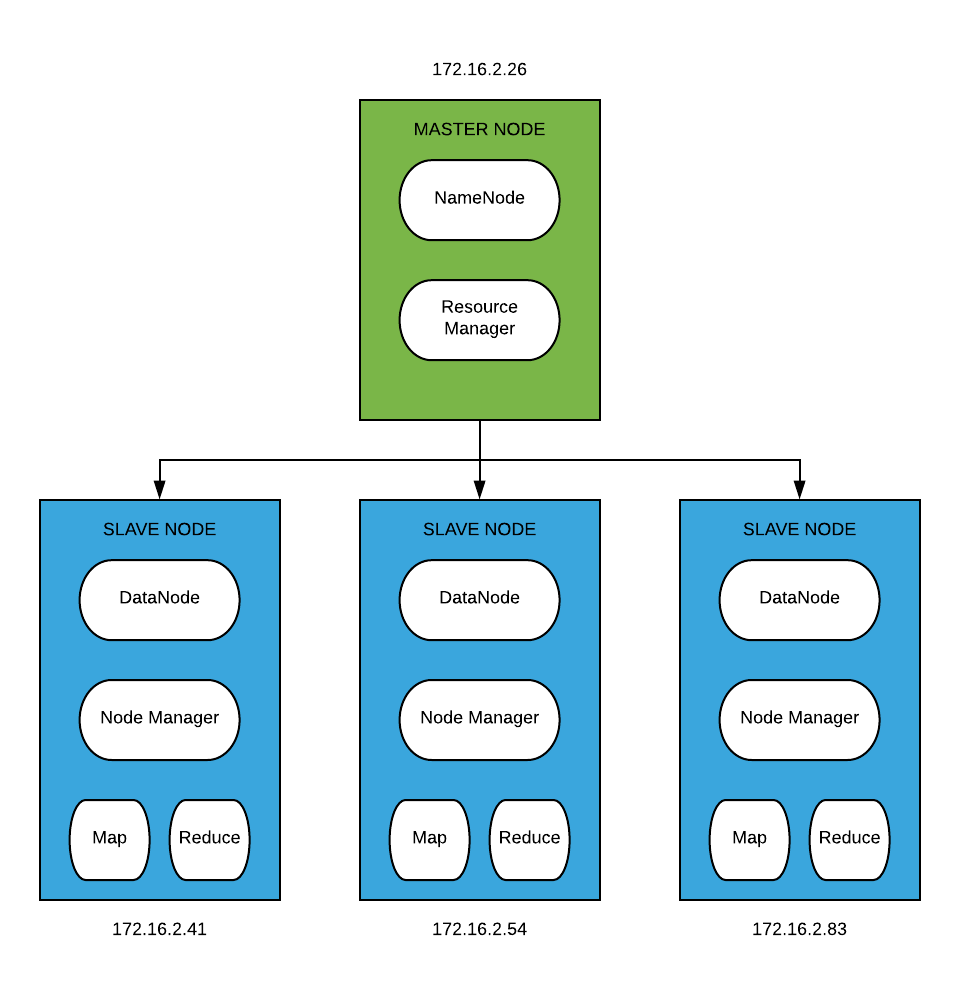
\includegraphics[width=10cm]{Hadoop-Diagram}
        \centering
        \caption{Hadoop Diagram}
    \end{figure}
   
\chapter{Implementation}\label{chap:implementation}
    
    \section{Pseudocode}
    \paragraph{}

    \clearpage
    \subsection{Kmeans Algorithm}
    \paragraph{}

    \begin{algorithm}[H]
        \SetAlgoLined
        \KwResult{The k-means algorithm using distributed computation}
        \SetKwInOut{Input}{input}\SetKwInOut{Output}{output}
        \Input{
            \\ $dataset$: Dataset File name with the complete path\;
            \\ $k$: Number of Clusters\;
            \\ $dimension$: Number of coordinates to work with\;
            \\ $threshold$: Value for flexibility of the convergence\;
            \\ $centroids$: Centroids File Name with the complete path\;
            \\ $output$: Output File Name to save the clusters\;
        }
        \Output{The set of mean $centroids$ that make the algorithm converged}
        \BlankLine
        parse the $input$ arguments\;
        $convergedCentroids\leftarrow 0$\;
        $iterations\leftarrow 0$\;
        $centroids\leftarrow$ set the initial random $centroids$ from the whole $dataset$\;
        \While{$convergedCentroids$  $<$ k}{
            \If{$iteration$ $>$ 0}{
                $centroids\leftarrow$ previous mean $centroids$\;
            }
            MAP every point and assign the closest centroid to it  \\
            REDUCE to find the mean centroid of each cluster   \\
            $convergedCentroids\leftarrow$ count of mean centroids that converged\;
            $iteration\leftarrow  iteration + 1$\;
        }
        \Return{convergedCentroids}\;
        \caption{$kMeans(dataset, k, dimension, threshold, centroids, output)$}
    \end{algorithm}
    
    \clearpage
    \subsection{Map Algorithm}
    \paragraph{}

    \begin{algorithm}[H]
        \SetAlgoLined
        \KwResult{Map every point and assign the closest centroid to it}
        \SetKwInOut{Input}{input}\SetKwInOut{Output}{output}
        \Input{
            \\ $line$: one row on the Dataset text file\;
        }
        \BlankLine
        $point\leftarrow new $ empty $ array$\;
        $coordinates$: split $line$ string by $","$\;
        $coordinateCounter\leftarrow 0$ \;
        \ForEach{$coordinate$  $in$ $coordinates$}{
            \If{$coordinateCounter$ $==$ dimension}{
                $break$\;
            }
            $value$: convert coordinate to double\;
            add $value$ to $point$\;
        }
        $closestCentroid\leftarrow empty$\;
        $minimumDistance\leftarrow infinity$\; 
        \ForEach{$centroid$  $in$ $centroids$}{
            $distance$: find $euclidean$ distance between $centroid$ and $point$\;
            \If{$distance$ $<$ minimumDistance}{
                $closestCentroid\leftarrow centroid$\;
                $minimumDistance\leftarrow distance$\;
            }
        }
        $EMIT(closestCentroid, point)$\;
        \caption{$MAP(line)$}
    \end{algorithm}

    \clearpage
    \subsection{Reduce Algorithm}
    \paragraph{}

    \begin{algorithm}[H]
    \SetAlgoLined
    \KwResult{Reduce to find the mean centroid of each cluster}
    \SetKwInOut{Input}{input}\SetKwInOut{Output}{output}
    \Input{
        \\ $centroid$: Current centroid \;
        \\ $values$: List of points assigned to centroid \;
    }
    \BlankLine
    $meanCentroid\leftarrow new$ empty $Array$ with the same dimension initialized to 0\;
    \ForEach{$point$ in $values$}{\label{forins}  
        update $meanCentroid$ by sum each element to $meanCentroid$ \;
        $EMIT(centroid, point)$\;
    }
    $meanCentroid\leftarrow$ dividing the meanCentroid by number of $elements$ in $values$\;
    $distance$:  $euclidean$ between $centroid$ and the $meanCentroid$\;
    \If{$distance$ $<=$ $threshold$}{
        $convergedCentroids\leftarrow  convergedCentroids + 1$\;
    }
    \caption{$REDUCE(centroid, values)$}
    \end{algorithm}

    \section{K-means in Hadoop}
    \paragraph{}
    
    \subsection{How to select random centroids in Hadoop?}
    \paragraph{}

    To choose initial random centroids, we used a MapReduce solution that exploits the sorter functionalities.  

    Initially, the mapper receives as input a text line and outputs each line with a random integer as key. 

    \subsection{Map in Hadoop Algorithm}
    \paragraph{}

    \begin{algorithm}[H]
        \SetAlgoLined
        \KwResult{Map every point and assign the closest centroid to it}
        \SetKwInOut{Input}{input}\SetKwInOut{Output}{output}
        \Input{
            \\ $line$: one row on the Dataset text file\;
        }
        \BlankLine
        $id$: set random number\;
        $EMIT(id, line)$\;
         \caption{$MAP(line)$}
    \end{algorithm}
    
    \clearpage
    \subsection{Reduce in Hadoop Algorithm}
    \paragraph{}

    \begin{algorithm}[H]
        \SetAlgoLined
        \KwResult{Reduce to find the mean centroid of each cluster}
        \SetKwInOut{Input}{input}\SetKwInOut{Output}{output}
        \Input{
            \\ $id$: is the id of the current centroid\;
            \\ $value$: is an array of points assigned to the centroid \;
        }
        \BlankLine
        parse the $input$ arguments\;
        $centroidsList$: set empy $list$\;
        \BlankLine
            \AlCapSty{\AlCapFnt setup:}\\
        $dimension, k\leftarrow$ get values from configuration\;
        $reduce(id, values)$\;
        \ForEach{$element$  $in$ $values$}{
            $point\leftarrow$ get a slice from element's array of the same size of dimension\;
            add $point$ to $centroidsList$\;
            $EMIT(null, point)$\;
            \If{$centroidsList$ $size ==$ k}{
                $break$\;
            }
        }
        \BlankLine
        \AlCapSty{\AlCapFnt cleanup:}\\
        $centroidsFile$: get $value$ from $configuration$\;
        \ForEach{$element$  $in$ $centroidsList$}{
            write $element$ in $centroidsFile$\; 
        }
        \caption{$REDUCE(id, values)$}
    \end{algorithm}

    Finally, the reducer outputs the first K values, throwing away the keys. 

    \clearpage
    \subsection{Job}
    \paragraph{}

    The steps below explains how a MapReduce job is created for processing a kmeans iteration: 

    \begin{figure}[H]
        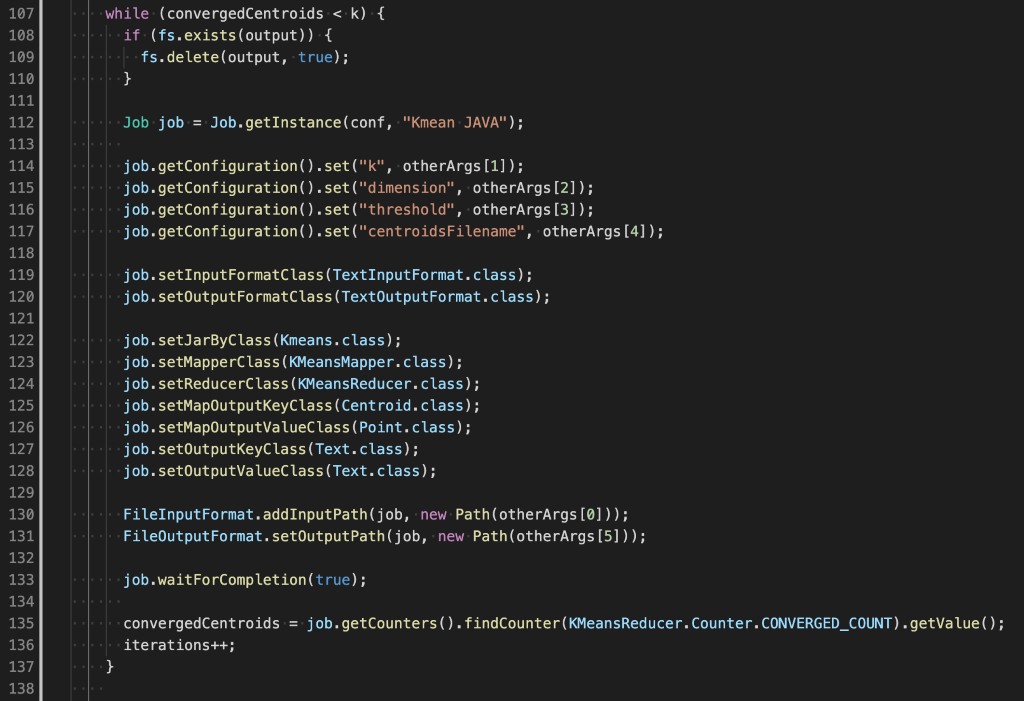
\includegraphics[width=12cm]{code/converged_centroids}
        \centering
        \caption{Kmeans iteration}
    \end{figure}

    \begin{enumerate}
        \item \textbf{From line 114 to 117:} we pass the required configuration to the job. 
        \item \textbf{From line 119 to 131:} we configure various job-specific parameters. 
        \item \textbf{Line 133:} Submits the job, then polls for progress until the job is complete.
        \item \textbf{Line 135:} is very important to evaluate the continuity of the process. If the number of converged centroids is less than \textit{k}, all the job will be started again. 
    \end{enumerate}

    \subsection{Map}

    At the beginning of the task we use the setup function as a preliminary phase where we retrieve the previous centroids in a file. 
    
    \begin{figure}[H]
        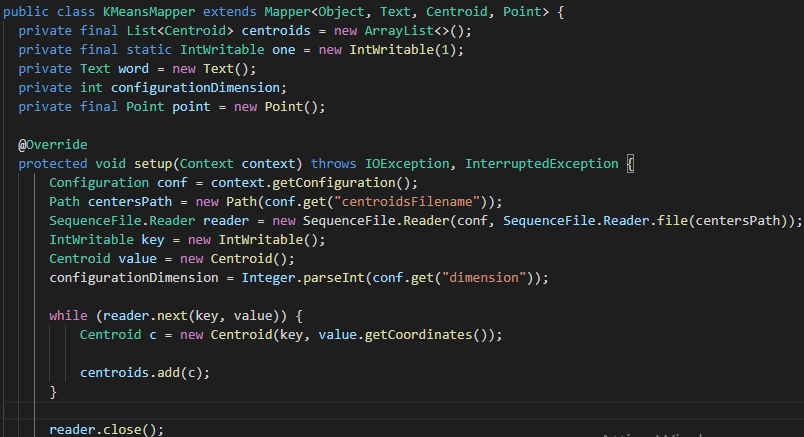
\includegraphics[width=12cm]{code/kMeansMapper}
        \centering
        \caption{KmeansMapper function in Hadoop}
    \end{figure}

    The filename where the centroids are located is taken from the centroidsFilename variable in the configuration passed to the job. 

    \begin{figure}[H]
        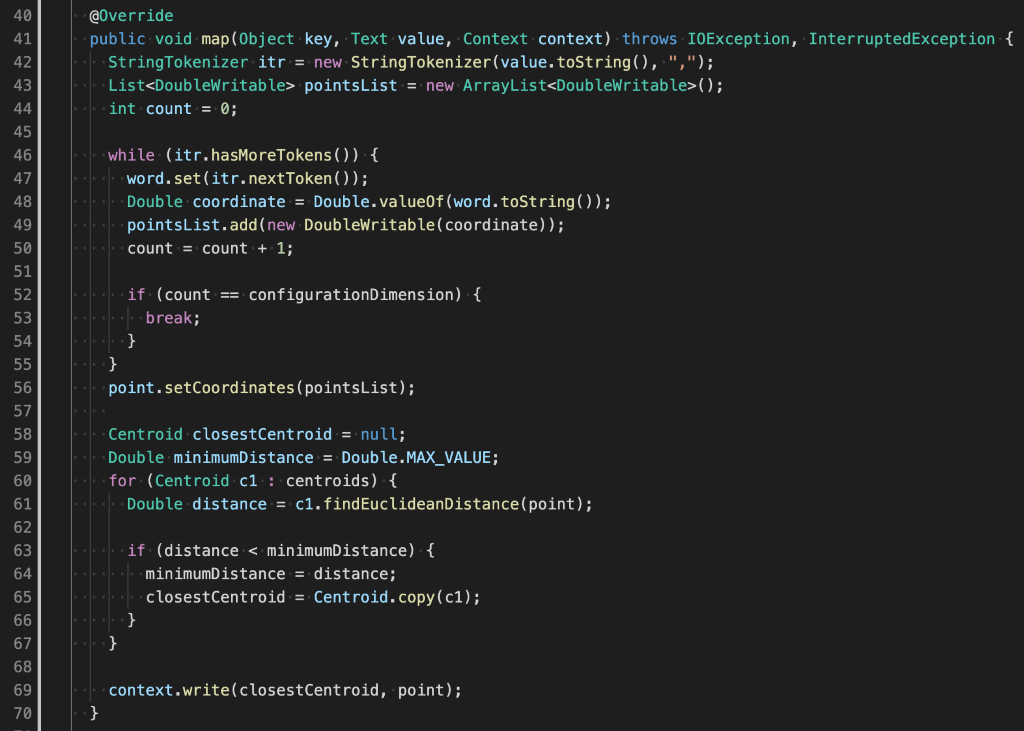
\includegraphics[width=12cm]{code/map}
        \centering
        \caption{Map function in Hadoop}
    \end{figure}

    \begin{enumerate}
        \item \textbf{From line 42 to line 56:} we splits a text line read from the file text to create a list, which is later used as coordinates for a point Object. 
        \item \textbf{From line 58 to line 69:} we compare the euclidean distance between the point and each centroid to find the closest centroid. 
    \end{enumerate}

    \subsection{Reduce}
    \paragraph{}
    
    The setup function \textit{(line 26)} in the reducer, similarly to the mapper function, preprocesses data needed for the following steps with the difference that it retrieves the dimension and the threshold from the Configuration.

    \begin{figure}[H]
        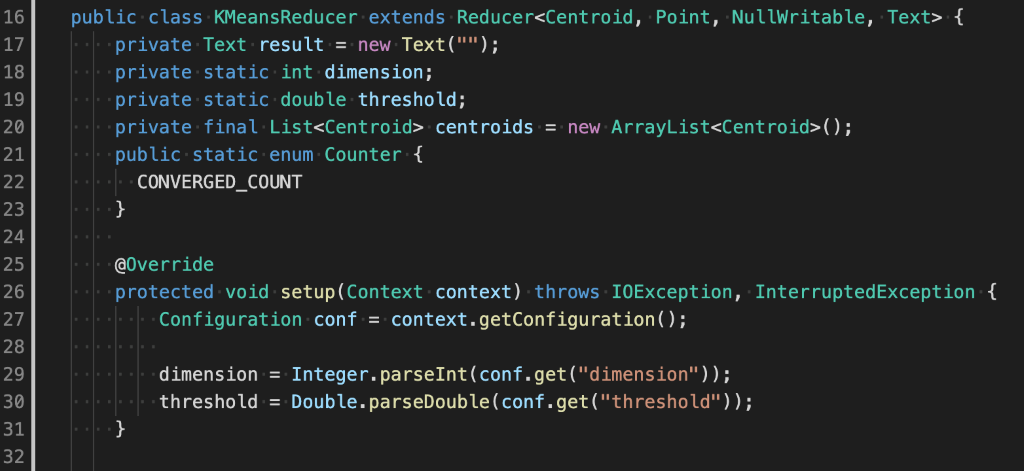
\includegraphics[width=12cm]{code/KmeansReducer}
        \centering
        \caption{KmeansReducer function in Hadoop}
    \end{figure}

    \begin{figure}[H]
        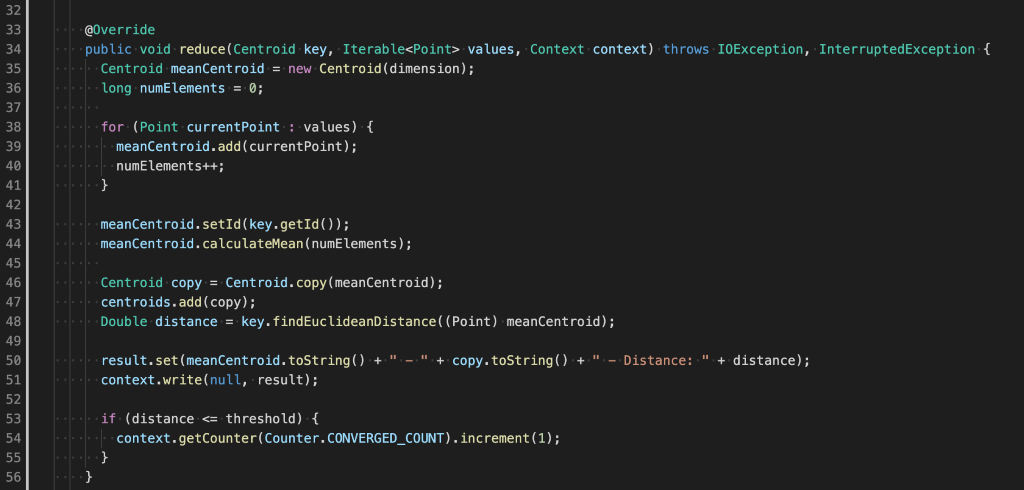
\includegraphics[width=12cm]{code/reduce}
        \centering
        \caption{Reduce function in Hadoop}
    \end{figure}

    \begin{enumerate}
        \item \textbf{From line 35 to line 44:} we calculate the mean centroid using the points received in the list of values of the reducer. 
        \item \textbf{From line 46 to line 55:} in the second part of the code, we calculate the distance between the mean centroid and the current centroid to check if the convergence respects the threshold. Therefore, if the condition of the convergence is respected we will increment the counter of the convergence. 
    \end{enumerate}

    The following code explains the cleanup function, where the program loops the mean centroids and writes them into a file for the next iteration. 

    \begin{figure}[H]
        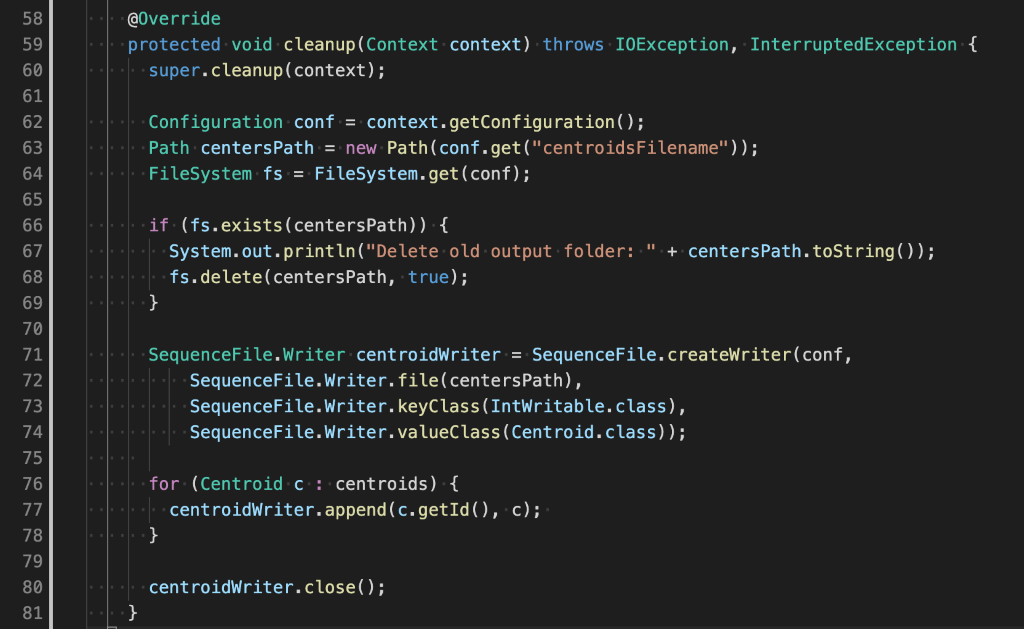
\includegraphics[width=12cm]{code/cleanup}
        \centering
        \caption{Cleanup function}
    \end{figure}

    \section{K-means in Spark}
    \paragraph{}

    \subsection{How to select random centroids in Spark?}
    \paragraph{}

    \begin{figure}[H]
        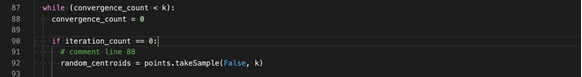
\includegraphics[width=12cm]{code/convergence_count_small}
        \centering
        \caption{Kmeans Spark}
    \end{figure}

    In the command \textbf{line 92} above we want to create a subset of RDD with fixed-size. The code has two parameters: 
    \begin{itemize}
        \item The first parameter specifies if we want to use replacement, In this case not, because we want unrepeated items. 
        \item The second parameter is the number of elements that we want, in our case \textbf{k} represents the number of initial centroids needed. 
    \end{itemize}

    \subsection{Spark Driver}
    \paragraph{}

   In line \textbf{76} we initialize the Spark Context that represents a connection with the master system. At the master argument we specifying \textit{yarn} because we want to connect to the yarn cluster. In the \textbf{lines 78 to line 81} we parse the argument values. 

    \begin{figure}[H]
        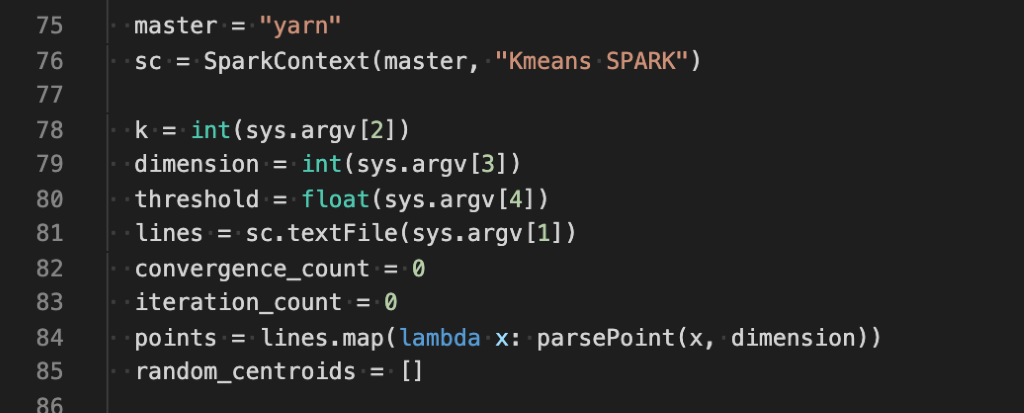
\includegraphics[width=12cm]{code/kmeans-spark}
        \centering
        \caption{Yarn Kmeans Spark}
    \end{figure}

	In the last section of the program \textbf{lines 87 to line 135} we run the job and evaluate if we need another iteration. In \textbf{line 110} we replaced the centroid with the mean previous one. 

    \begin{figure}[H]
        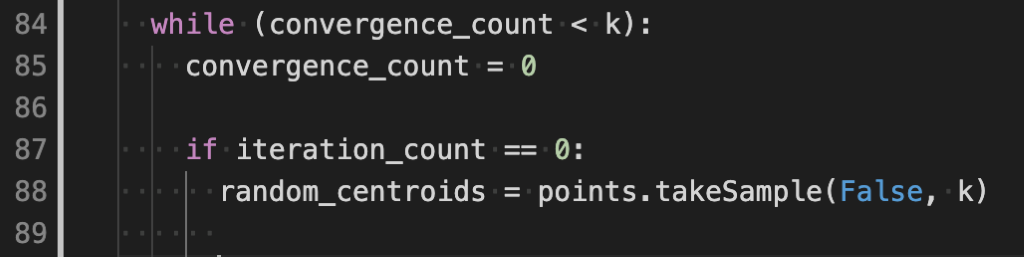
\includegraphics[width=12cm]{code/convergence_count}
        \centering
        \caption{Kmeans iteration}
    \end{figure}

    In the last section of the program \textbf{lines 71 to line 92} we run the job and evaluate if we need another iteration. In line 77 we replaced the centroid with the mean previous one. 

    \subsection{Map}
    \paragraph{}

    The Map function in Spark works in a different way. In the below picture \textbf{line 112}, We mapped the RDD of points taken from the file and called assign\_nearest\_centroid to each point. 

    \begin{figure}[H]
        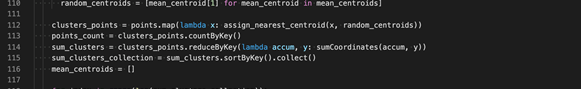
\includegraphics[width=12cm]{code/random_centroids_small}
        \centering
        \caption{Map function in Spark}
    \end{figure}

    The following function is the same process as \textbf{line 58 to line 69} in the java solution. 

    \begin{figure}[H]
        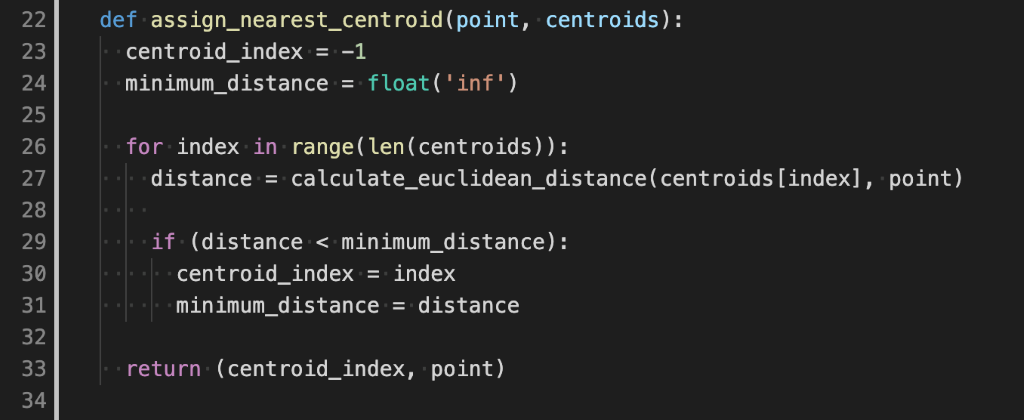
\includegraphics[width=12cm]{code/nearest_centroid}
        \centering
        \caption{Nearest Centroid function in Spark}
    \end{figure}

    \subsection{Reduce}
    \paragraph{}

    The reduce function is in the line 92 and basically it groups the points by the key values, which are the nearest cluster. 
    
    \begin{figure}[H]
        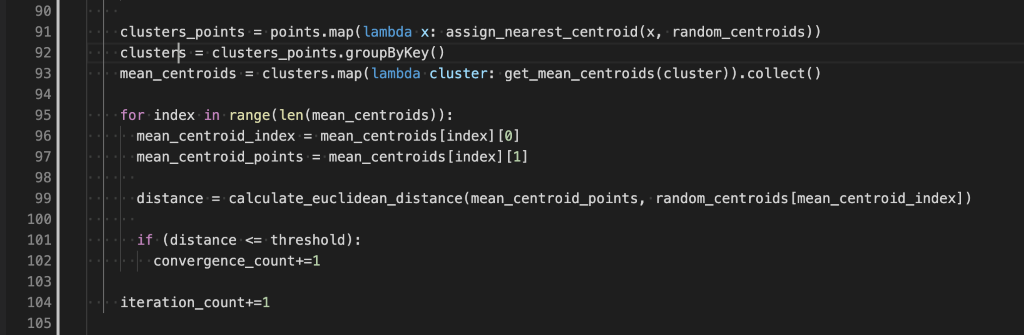
\includegraphics[width=12cm]{code/cluster_points}
        \centering
        \caption{Reduce function in Spark}
    \end{figure}

    In the line 93 we process the mean centroid of each cluster using the map function.  

    Eventually, we compute the euclidian distance between the mean centroid and the previous centroid using a threshold. The condition of the convergence happens when the distance is less or equal of the threshold. If the condition is true the process continues to compute the distance by adding a unit to the convergence counter. Afterwards the process continue iteratively (iteration\_count+=1). 


\chapter{Experimental Results}\label{chap:experimental}
\paragraph{}
    Before to apply the k-means algorithms to our data, we have to fix the first centroids. They could be chosen in two different ways: 

    \begin{itemize}
        \item randomly way 
        \item prefixed way 
    \end{itemize}
        
    To understand better how \textbf{HADOOP} and \textbf{SPARK} works, we analyze them first, in a singular way choosing randomly centroids and then we will do a comparison between them choosing prefixed centroids which are the same for both the configuration. 
 
    \section{Hadoop}
    \paragraph{}

    \subsection{MapReduce with 1.000 points}
    \paragraph{}

    \begin{figure}[H]
        \hfill
        \subfigure[]{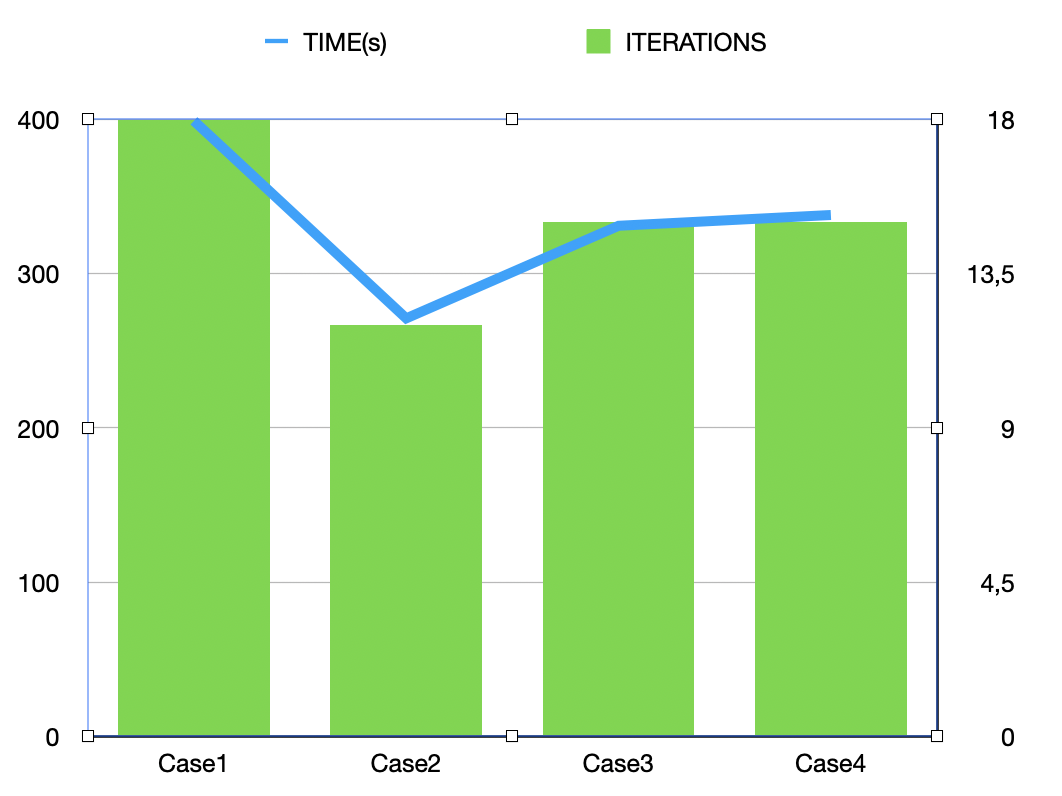
\includegraphics[width=4cm]{hadoop/grafico_1_point1k}}
        \hfill
        \subfigure[]{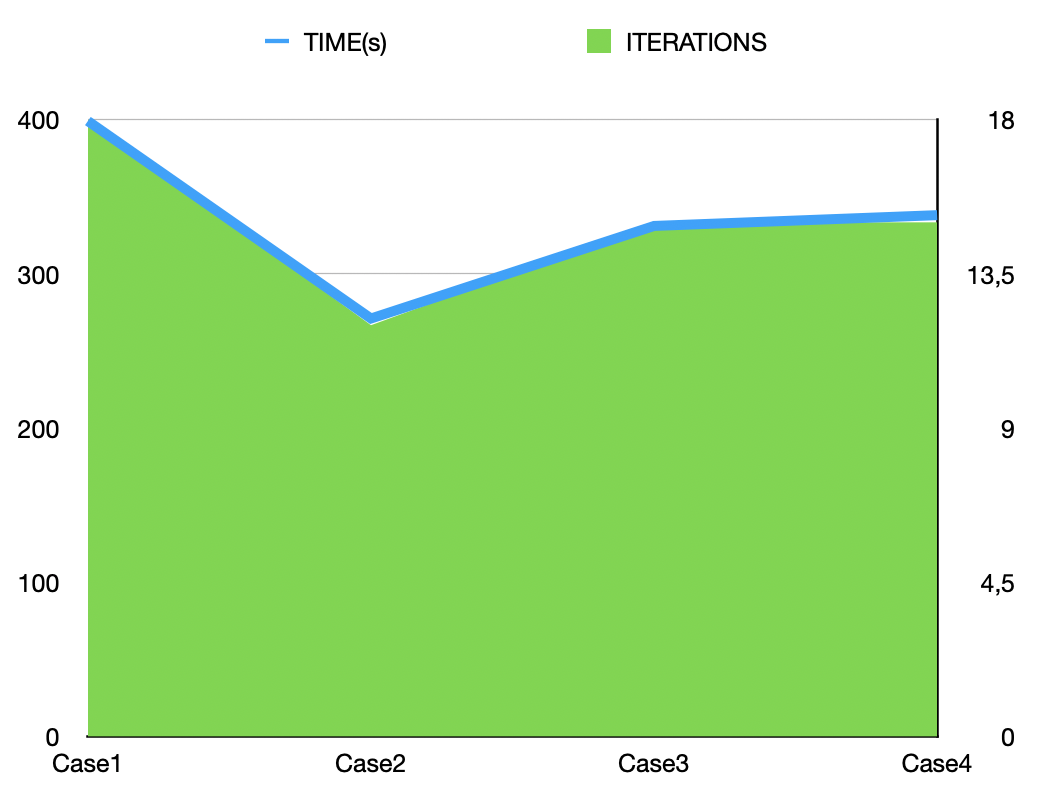
\includegraphics[width=4cm]{hadoop/grafico_2_point1k}}
        \hfill
        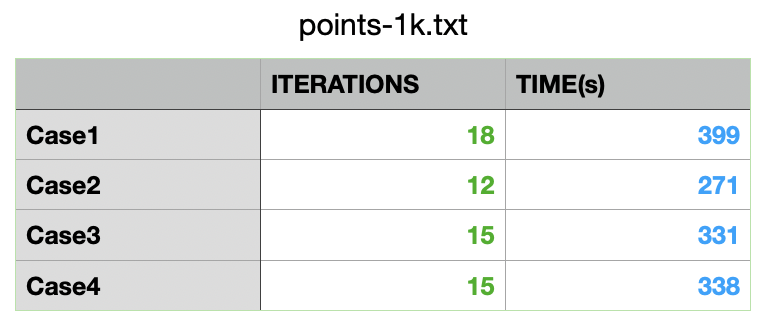
\includegraphics[width=5cm]{hadoop/tabella_point1k}
        \centering
        \caption{\footnotesize{\textbf{Case1:} d=3, k=7 \textbf{Case2:} d=3, k=13 \textbf{Case3:} d=7, k=7 \textbf{Case4:} d=7, k=13}}
    \end{figure}

    \subsection{MapReduce with 10.000 points}
    \paragraph{}

    \begin{figure}[H]
        \hfill
        \subfigure[]{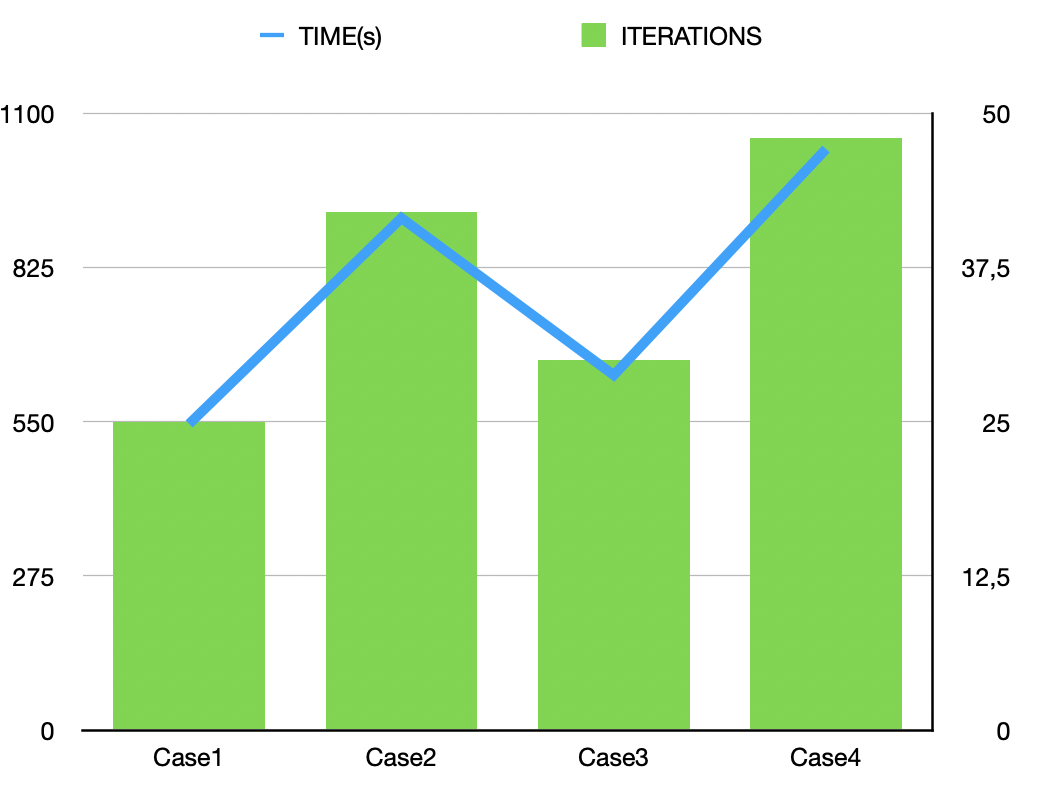
\includegraphics[width=4cm]{hadoop/grafico_1_point10k}}
        \hfill
        \subfigure[]{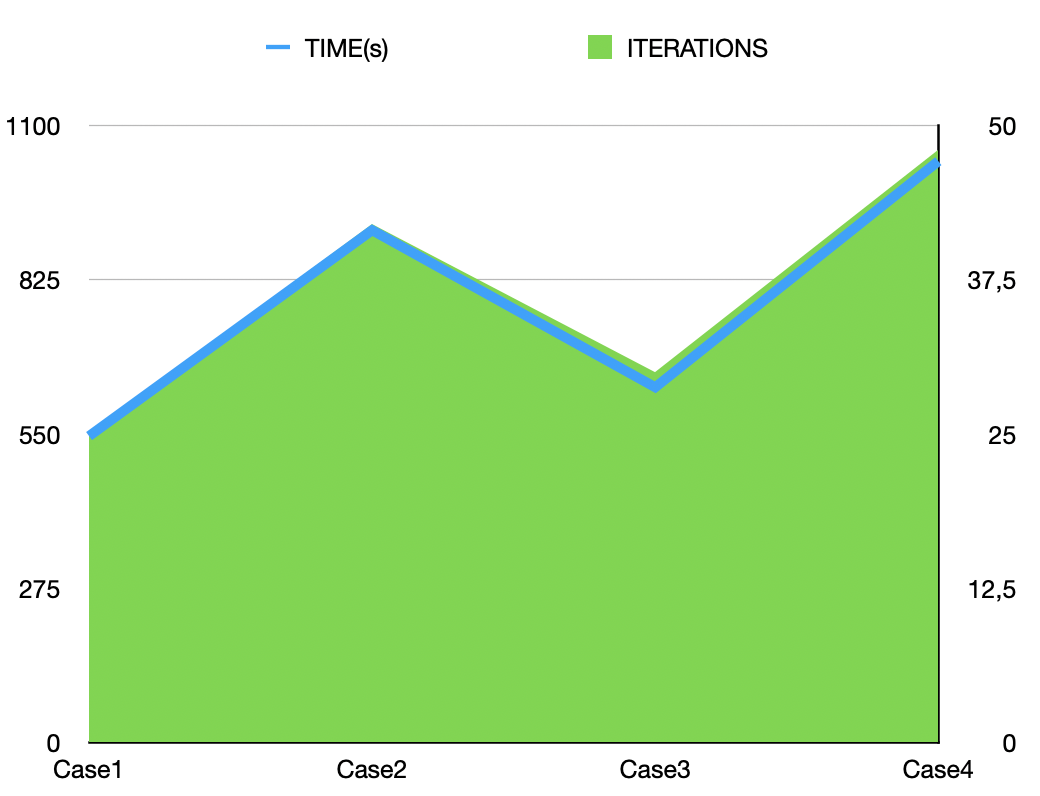
\includegraphics[width=4cm]{hadoop/grafico_2_point10k}}
        \hfill
        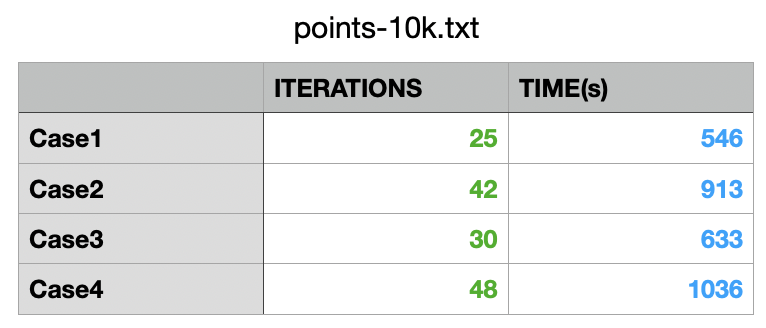
\includegraphics[width=5cm]{hadoop/tabella_point10k}
        \centering
        \caption{\footnotesize{\textbf{Case1:} d=3, k=7 \textbf{Case2:} d=3, k=13 \textbf{Case3:} d=7, k=7 \textbf{Case4:} d=7, k=13}}
    \end{figure}

    \subsection{MapReduce with 100.000 points}
    \paragraph{}

    \begin{figure}[H]
        \hfill
        \subfigure[]{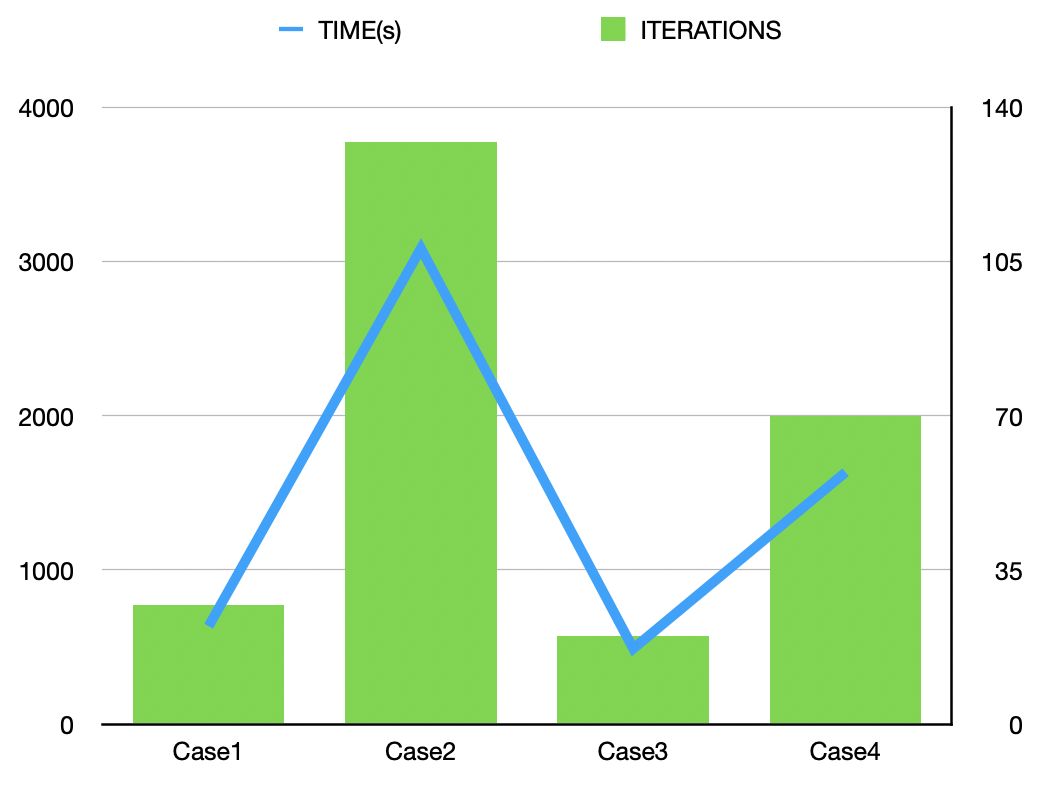
\includegraphics[width=4cm]{hadoop/grafico_1_point100k}}
        \hfill
        \subfigure[]{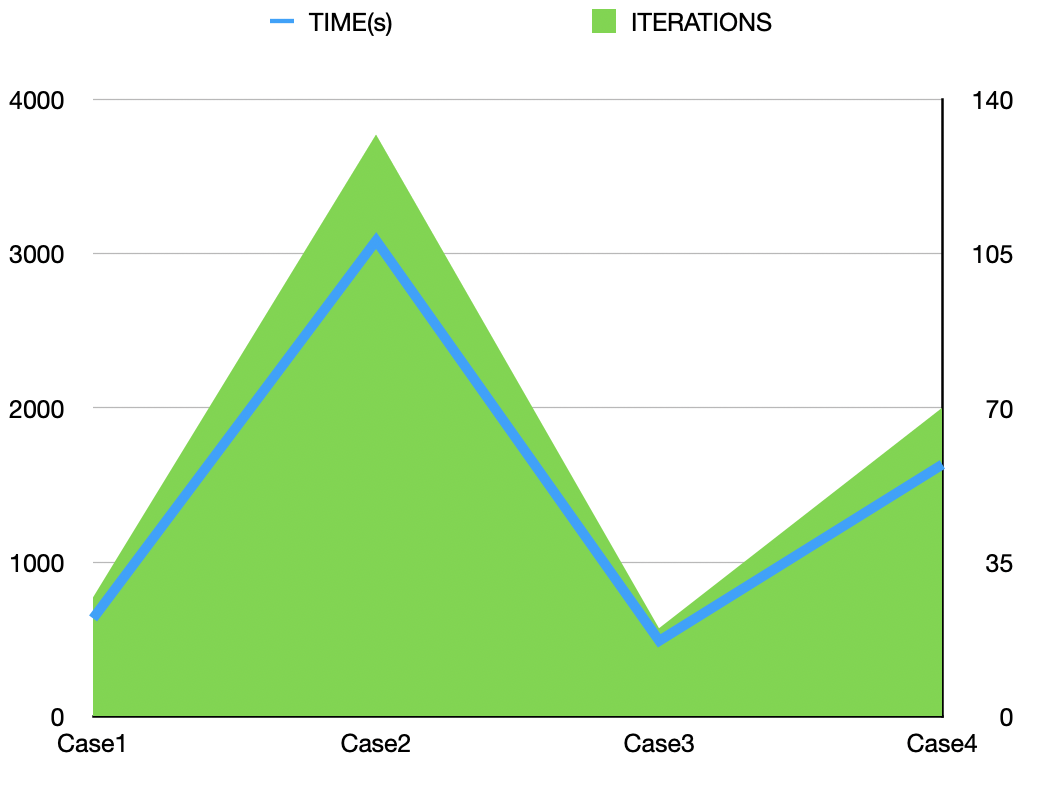
\includegraphics[width=4cm]{hadoop/grafico_2_point100k}}
        \hfill
        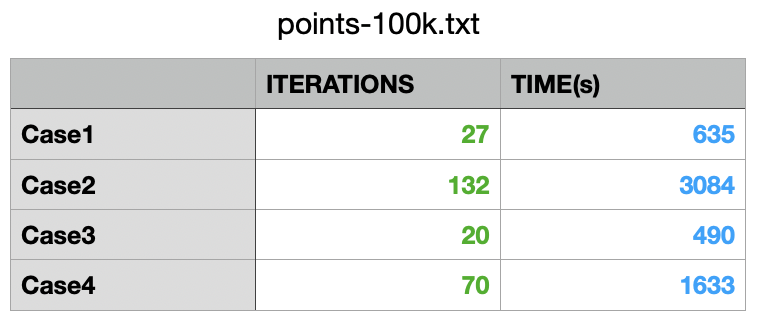
\includegraphics[width=5cm]{hadoop/tabella_point100k}
        \centering
        \caption{\footnotesize{\textbf{Case1:} d=3, k=7 \textbf{Case2:} d=3, k=13 \textbf{Case3:} d=7, k=7 \textbf{Case4:} d=7, k=13}}
    \end{figure}

    \subsection{Results on Hadoop}
    \paragraph{}

    These are our experimental results of the Hadoop Map reduce where we have picked our centroids in a randomly way. As we can see, the times and the iterations are like linearly independent. In fact, they present the same gait: if the iterations grow, time also increase. We could analyze better the last case where we have the maximum dataset. In the last scenario time grows as soon as the number of iterations increase but, the time (line in blue) is below the iterations (area in green) due to the fact that Hadoop works better with a huge amount of data. 

    \section{Spark}
    \paragraph{}

    \subsection{MapReduce with 1.000 points}
    \paragraph{}

    \begin{figure}[H]
        \hfill
        \subfigure[]{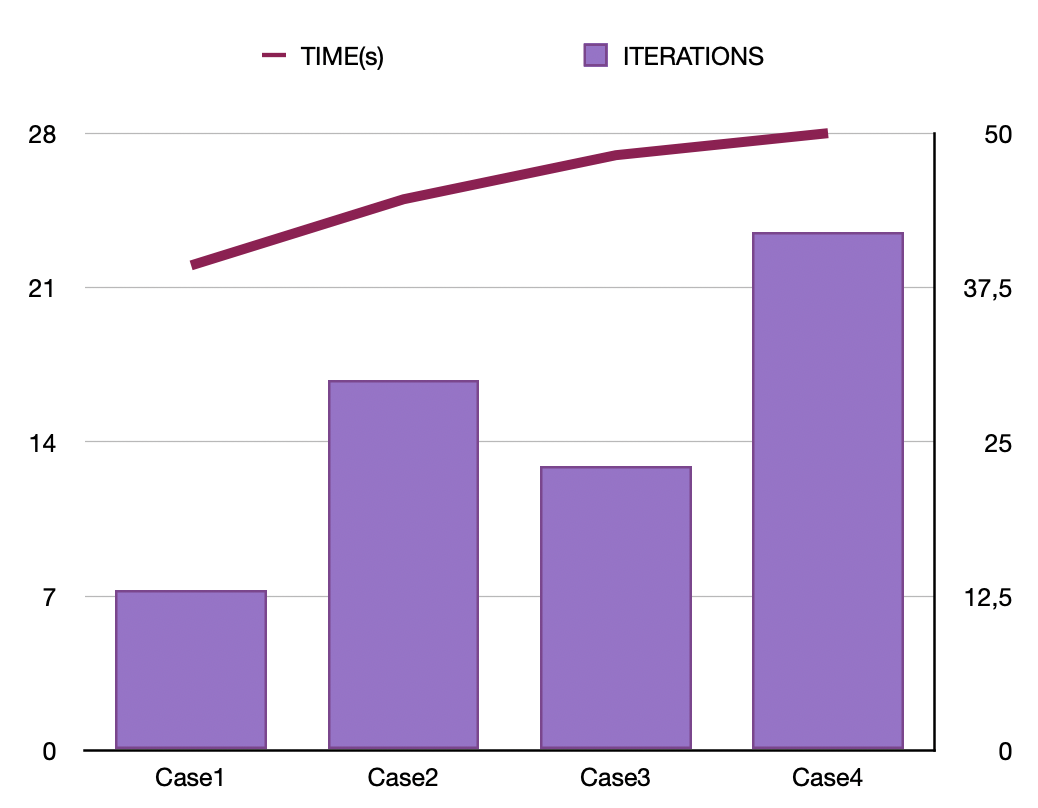
\includegraphics[width=4cm]{spark/grafico_1_point1k}}
        \hfill
        \subfigure[]{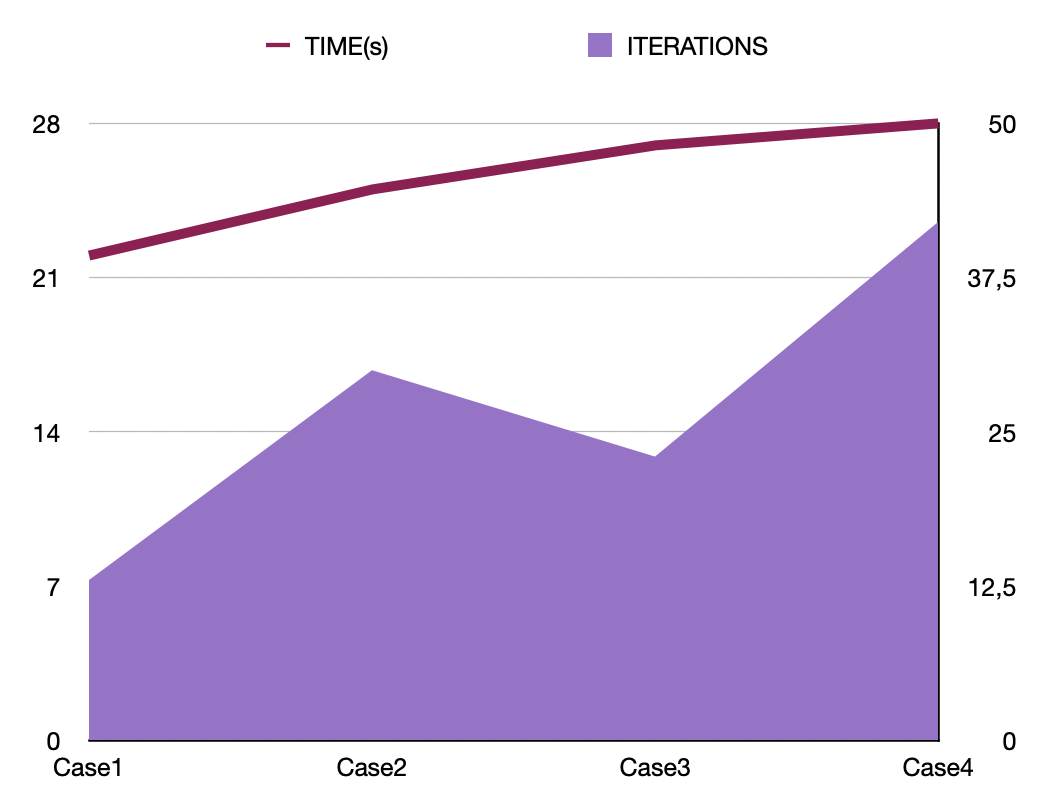
\includegraphics[width=4cm]{spark/grafico_2_point1k}}
        \hfill
        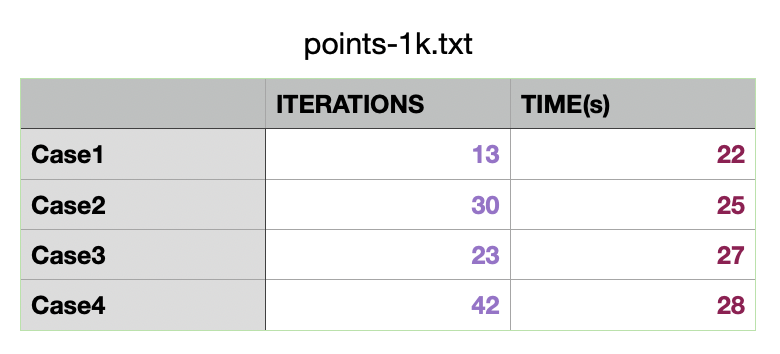
\includegraphics[width=5cm]{spark/tabella_point1k}
        \centering
        \caption{\footnotesize{\textbf{Case1:} d=3, k=7 \textbf{Case2:} d=3, k=13 \textbf{Case3:} d=7, k=7 \textbf{Case4:} d=7, k=13}}
    \end{figure}

    \subsection{MapReduce with 10.000 points}
    \paragraph{}

    \begin{figure}[H]
        \hfill
        \subfigure[]{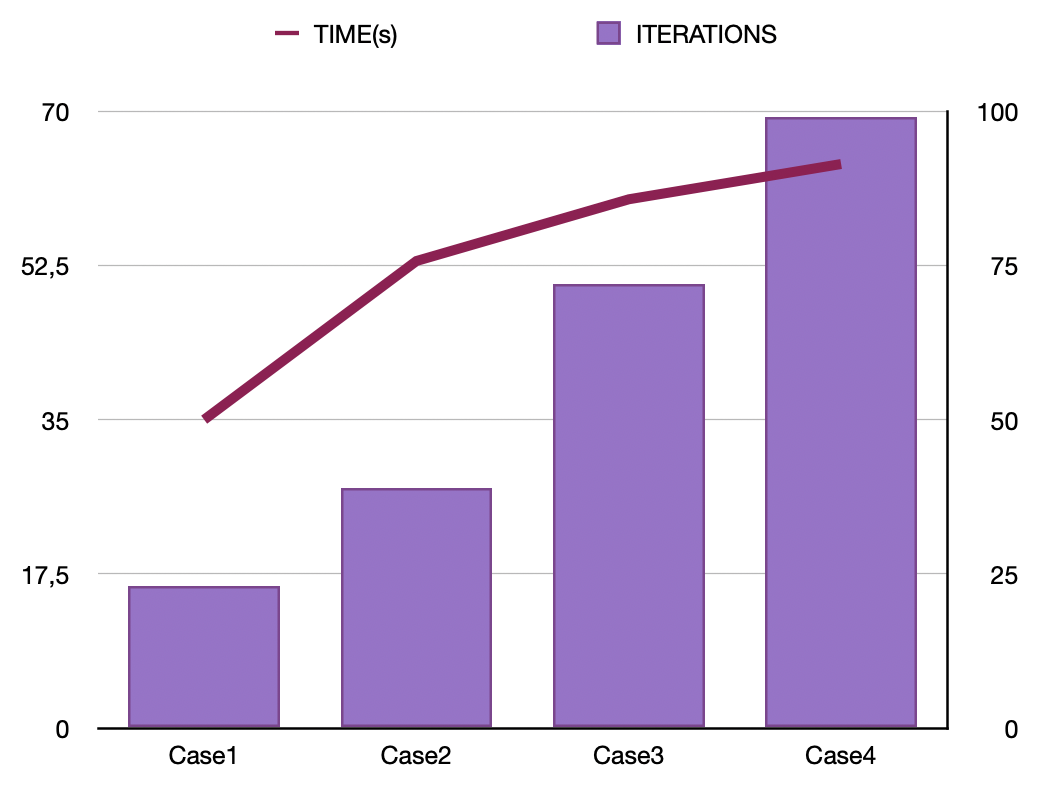
\includegraphics[width=4cm]{spark/grafico_1_point10k}}
        \hfill
        \subfigure[]{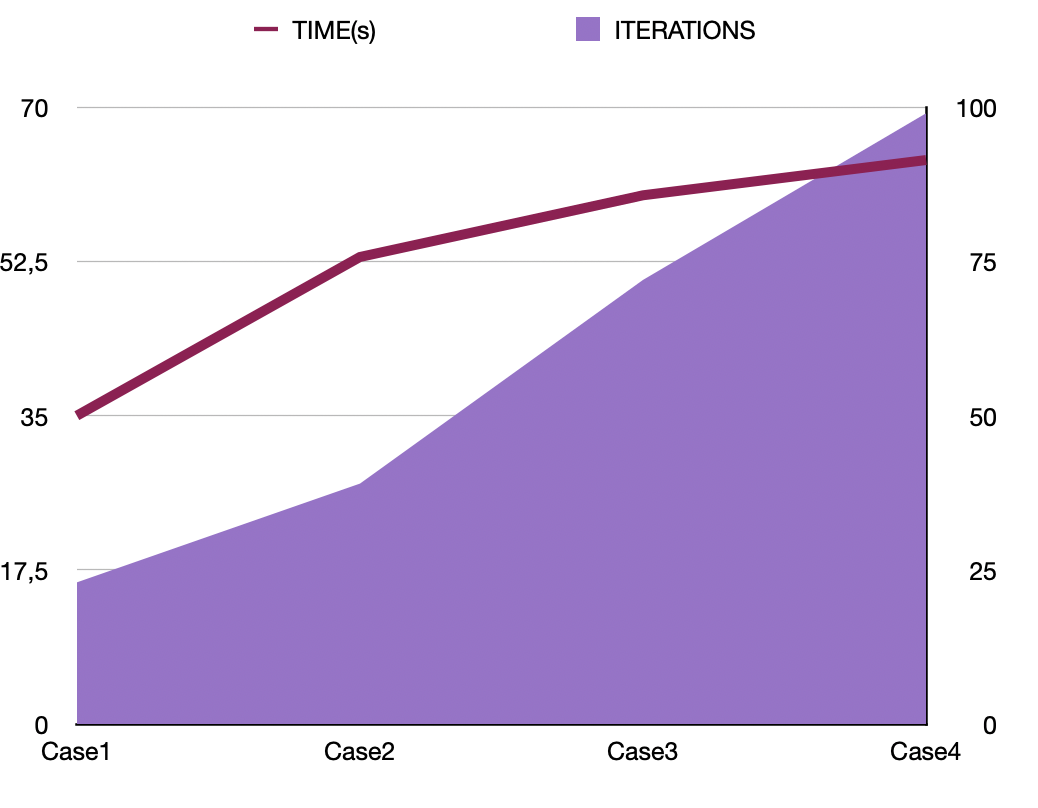
\includegraphics[width=4cm]{spark/grafico_2_point10k}}
        \hfill
        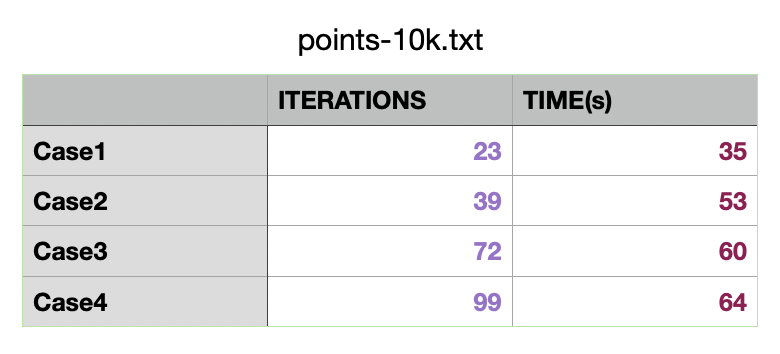
\includegraphics[width=5cm]{spark/tabella_point10k}
        \centering
        \caption{\footnotesize{\textbf{Case1:} d=3, k=7 \textbf{Case2:} d=3, k=13 \textbf{Case3:} d=7, k=7 \textbf{Case4:} d=7, k=13}}
    \end{figure}

    \subsection{MapReduce with 100.000 points}
    \paragraph{}
     
    \begin{figure}[H]
        \hfill
        \subfigure[]{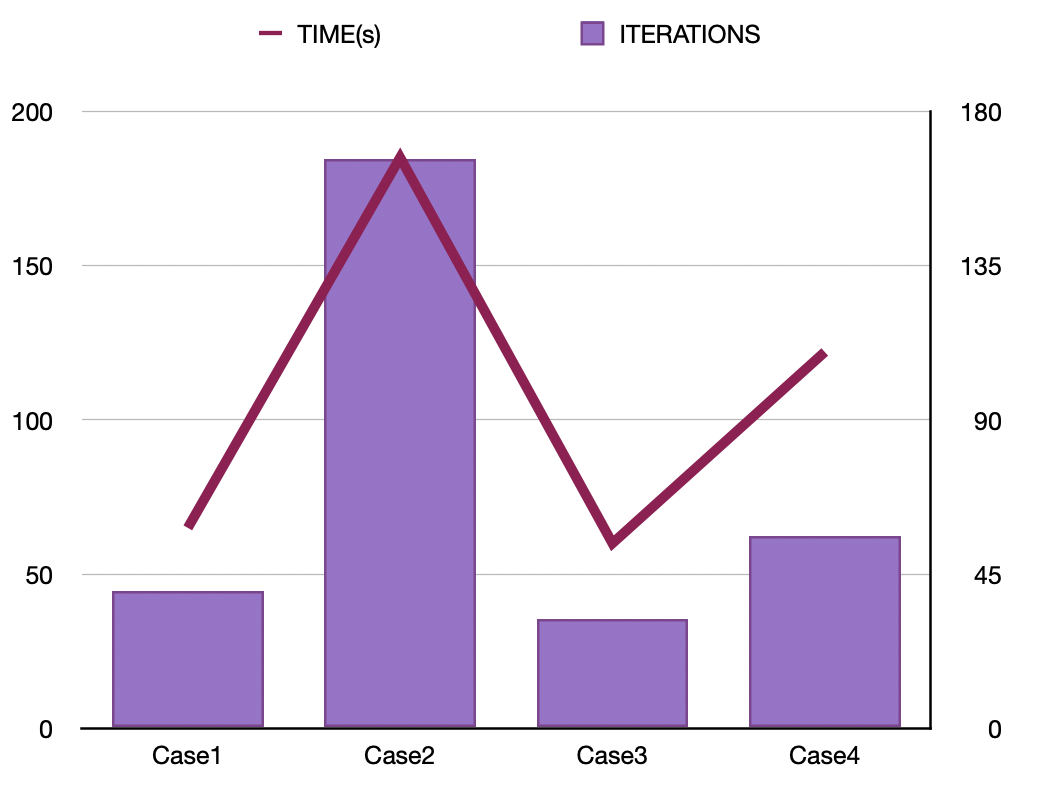
\includegraphics[width=4cm]{spark/grafico_1_point100k}}
        \hfill
        \subfigure[]{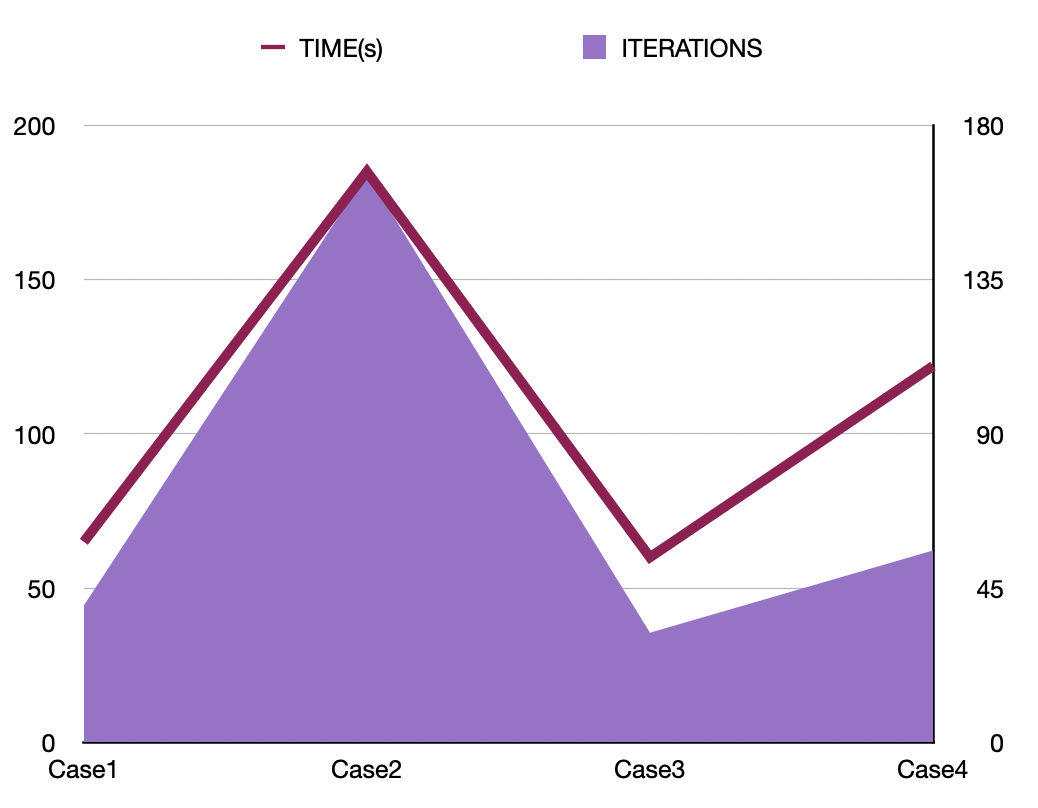
\includegraphics[width=4cm]{spark/grafico_2_point100k}}
        \hfill
        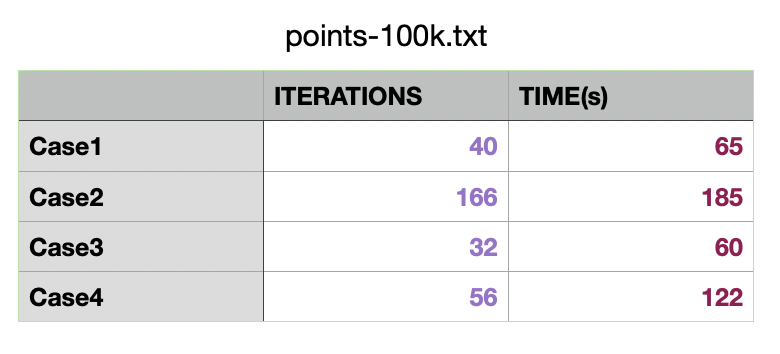
\includegraphics[width=5cm]{spark/tabella_point100k}
        \centering
        \caption{\footnotesize{\textbf{Case1:} d=3, k=7 \textbf{Case2:} d=3, k=13 \textbf{Case3:} d=7, k=7 \textbf{Case4:} d=7, k=13}}
    \end{figure}

    \subsection{Results on Spark}
    \paragraph{}
    These are our experimental results of the Spark Map reduce where we have picked our centroids in a randomly way. As we can see, the time grows in base of the number of iterations but in a constant way for the first two case because in this case the algorithm is too faster. Instead in the third case the time and the iterations present the same gait: if the iterations grow, time also increase and the time (line in brown) is above the iterations (area in purple), hence Spark works better with a small amount of data. 

    \section{Comparison of Spark and Hadoop}
    \paragraph{}

    \subsection{Time in seconds comparison with 1.000 points}
    \paragraph{}

    \begin{figure}[H]
        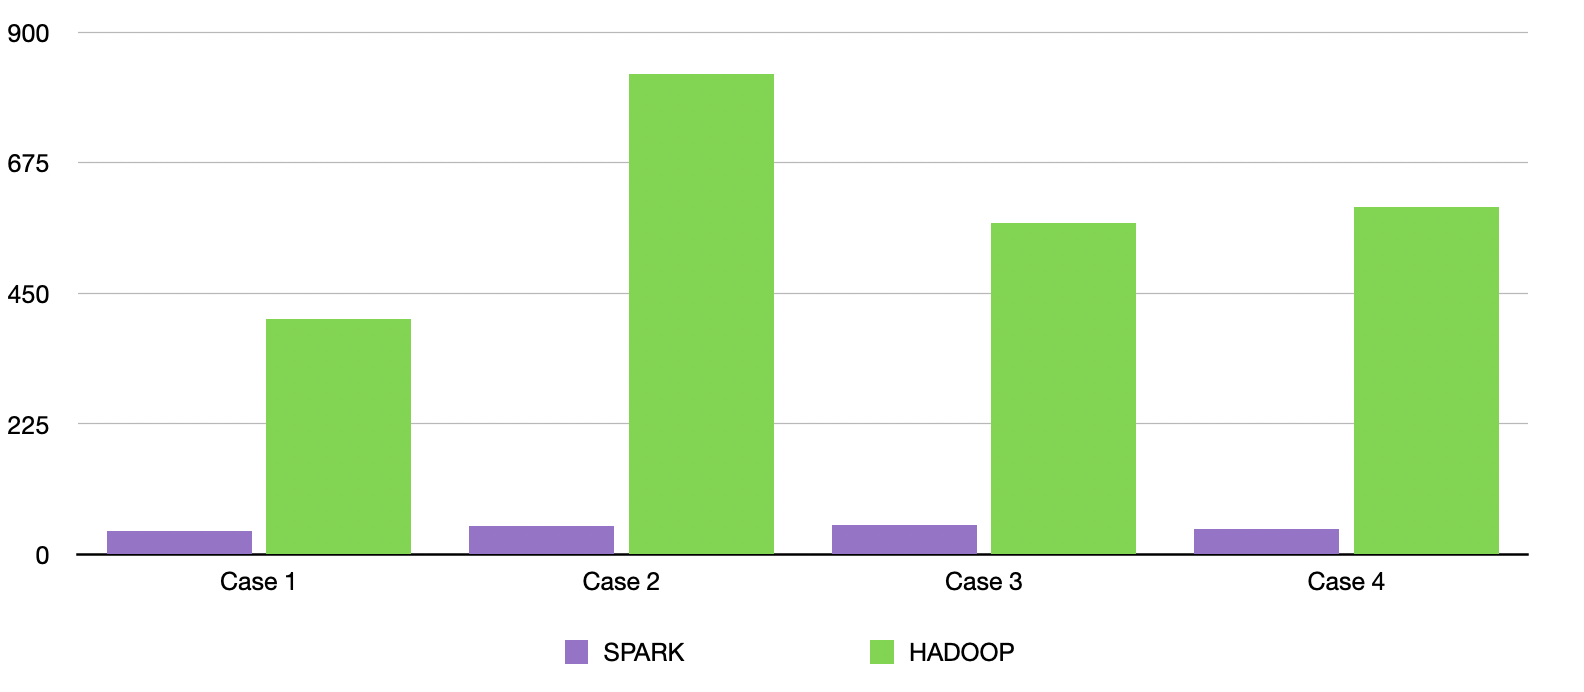
\includegraphics[width=10cm]{hadoop+spark/grafico_points1k}
        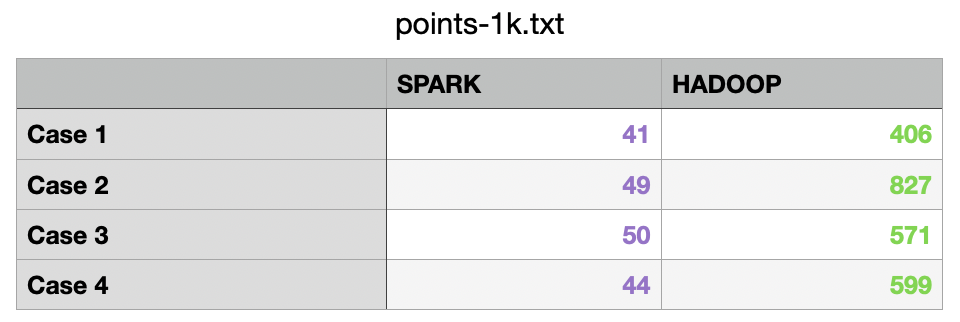
\includegraphics[width=5cm]{hadoop+spark/tabella_point1k}
        \centering
        \caption{\footnotesize{\textbf{Case1:} d=3, k=7 \textbf{Case2:} d=3, k=13 \textbf{Case3:} d=7, k=7 \textbf{Case4:} d=7, k=13}}
    \end{figure}


    \subsection{Time in seconds comparison with 10.000 points}
    \paragraph{}

    \begin{figure}[H]
        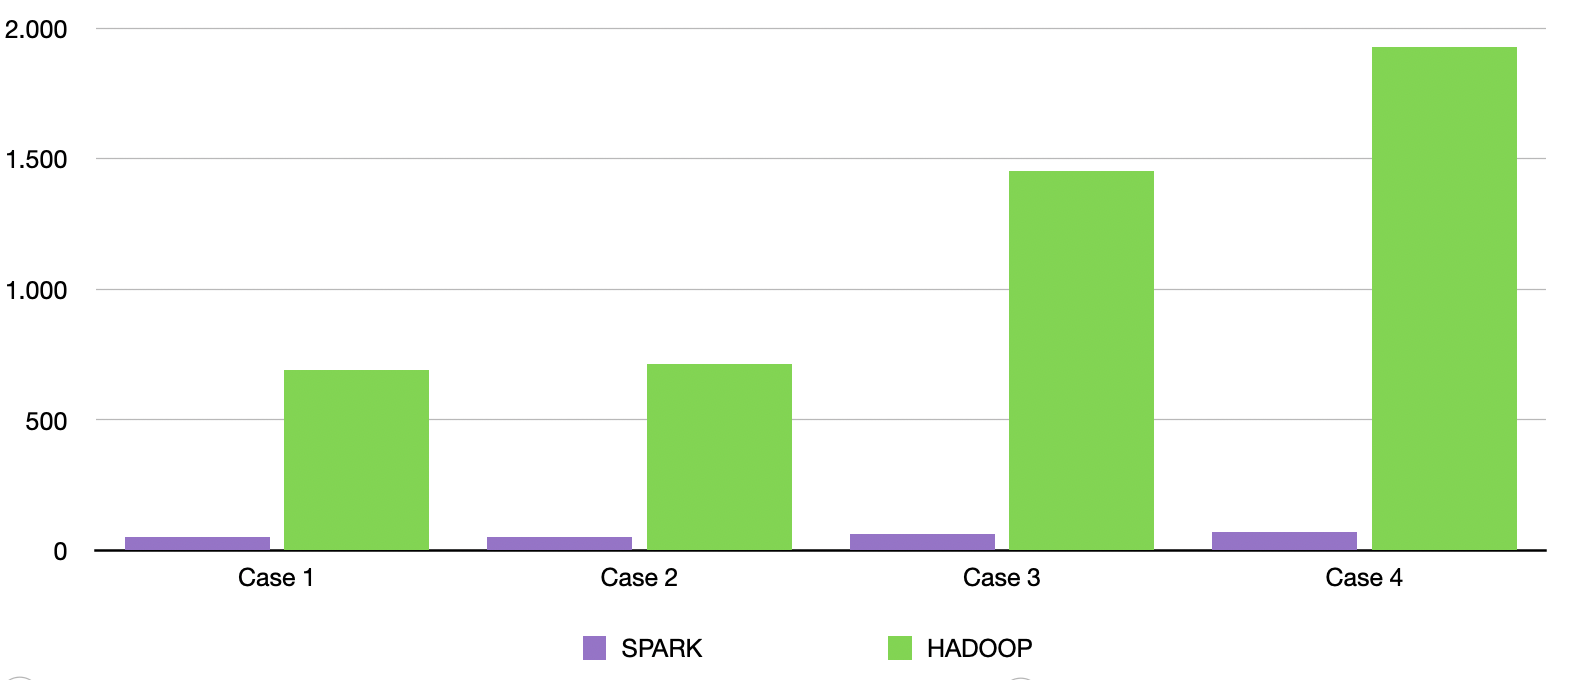
\includegraphics[width=10cm]{hadoop+spark/grafico_points10k}
        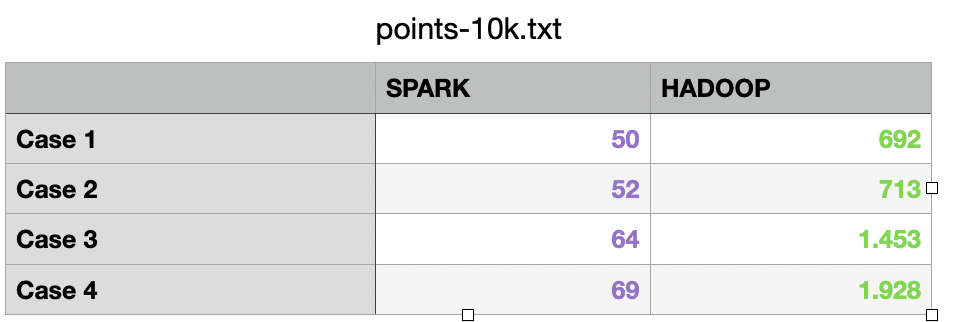
\includegraphics[width=5cm]{hadoop+spark/tabella_point10k}
        \centering
        \caption{\footnotesize{\textbf{Case1:} d=3, k=7 \textbf{Case2:} d=3, k=13 \textbf{Case3:} d=7, k=7 \textbf{Case4:} d=7, k=13}}
    \end{figure}


    \subsection{Time in seconds comparison with 100.000 points}
    \paragraph{}

    \begin{figure}[H]
        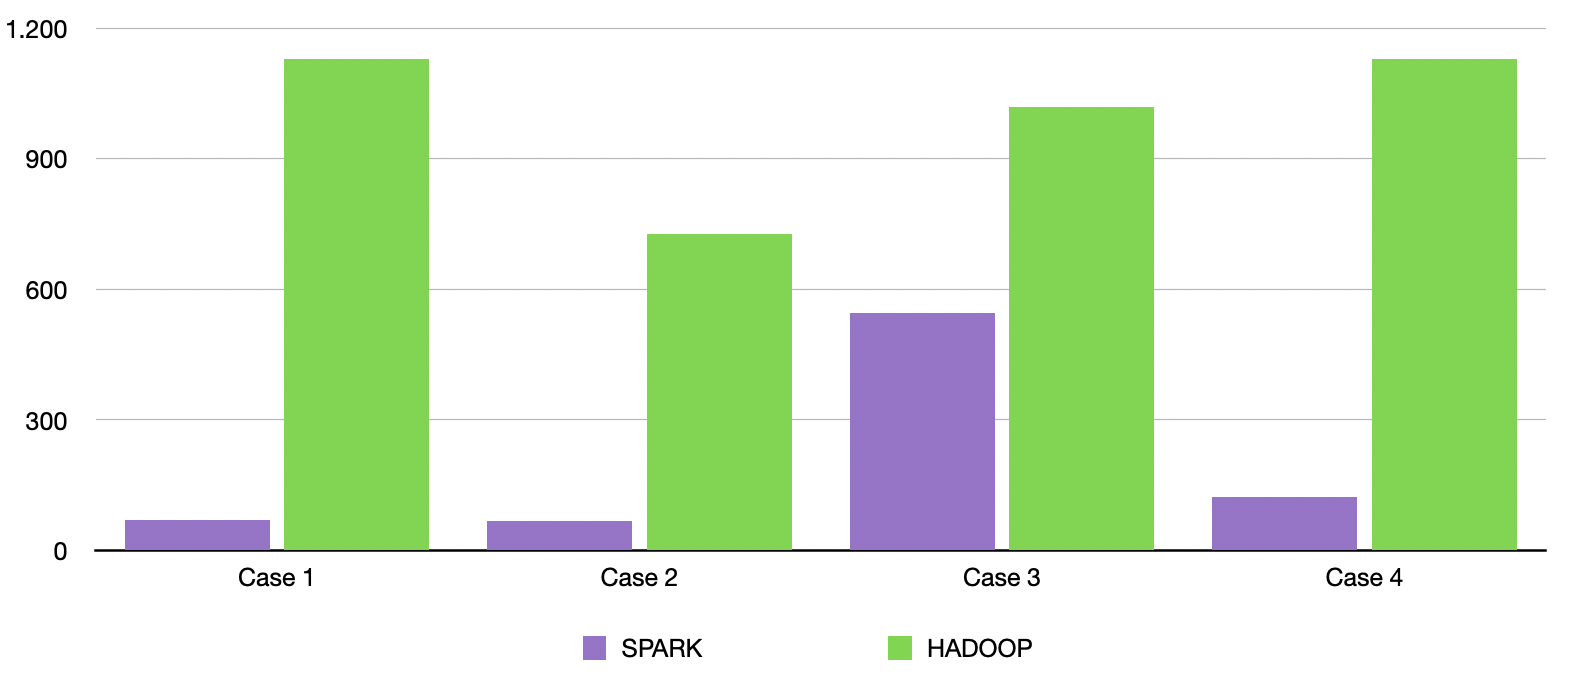
\includegraphics[width=10cm]{hadoop+spark/grafico_points100k}
        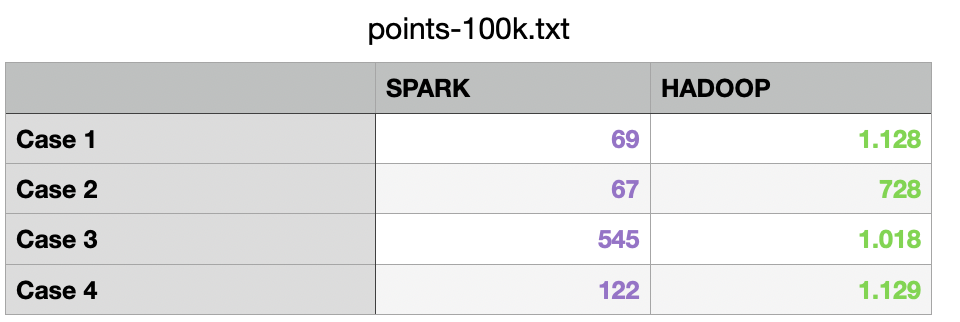
\includegraphics[width=5cm]{hadoop+spark/tabella_point100k}
        \centering
        \caption{\footnotesize{\textbf{Case1:} d=3, k=7 \textbf{Case2:} d=3, k=13 \textbf{Case3:} d=7, k=7 \textbf{Case4:} d=7, k=13}}
    \end{figure}

    \subsection{Results of the comparison of Hadoop and Spark}
    \paragraph{}

    To make a time comparison between Hadoop and Spark we need to fix the initial centroids to guarantee tests in same conditions; in fact, both the algorithms converge with the same number of iterations but different times. 

    In all three cases we could notice that the spark algorithm takes less time than Hadoop to converge and so it could be consider better in terms of time; but, if we analyze better the situation in which we have 100.000 points, in the case 3,  Spark algorithms takes more time than the other cases and it's because we have more iterations than others and that Spark does harder work with a huge amount of data. 

\chapter{Conclusions}\label{chap:experimental}
    \section{Key Difference between Hadoop MapReduce and Spark}
    \paragraph{}

	The key difference between Hadoop MapReduce and Spark lies in the approach to processing: Spark can do it in-memory, while Hadoop MapReduce must read from the memory and write to a disk. As a result, the speed of processing differs significantly and Spark may be up to 100 times faster. However, the volume of data processed also differs Hadoop MapReduce can work with far larger data sets than Spark. 

    Each iteration will be prolonged by I/O operations, which become a more relevant slow-down factor than the number of points inside the same configuration: the execution times in the Hadoop version do not change greatly with the size of the data set as occurs with Spark. 

    The results clearly showed that the performance of Spark turn out to be considerably higher in terms of time, where each of the dataset size results in a decrease in the processing time as compared to that of Map Reduce. 


    % Prints bibliography
    \printbibliography

\end{document}

